\section{Introduction}
The BraTS scans are 3D volumes. The groups participating in the BraTS contest build neural networks that work with these volumes as input directly.

One of the groups participating on the contest is the Healthcare Imaging A.I. group of the medical faculty of the University of Bern. The constituent of this thesis
is Mauricio Reyes, who is also the head of this group.

Applying the Hausdorff distance mask method on the neural network developed by the group could be helpful to enhance the neural network.

\subsection{Docker setup}
\nblink{brats3D/01\_preprocess.ipynb}

All participants of the contest are required to provide Docker images containing their neural networks. The Docker containers have to conform to a specific format which
was specified by the contest organizers. This simplifies the evaluation of the neural network, because all neural networks can be used in the same fashion.

The Docker container can only analyze a single scan at a time. When analyzing multiple scans, the container has to be executed again.

The Docker daemon mounts a directory from the host system into the container. The directory should contain the input files (4 files in the NIFTI format, one for each modality). The container will write the result (volume segment of the tumor, also in the NIFTI format) into the same directory.

The execution time to analyze a single scan varies from container to container. For CPU based neural network, it takes between 3 to 6 minutes to analyze one scan. GPU based networks take around one to two minutes.

\subsection{Zero out cubes}
\nblink{brats3D/02\_generate\_slices.ipynb}
The 2D version of the algorithm works by removing information by drawing a black circle onto the image. In the 3D version, we remove a small cube from the input files.
We load the NIFTI file, set a cubic part of the loaded 3D matrix to zero and save the scan again. An example of a modified volume is shown in Figure \ref{brats3d_example}.

\begin{figure}[H]
\centering
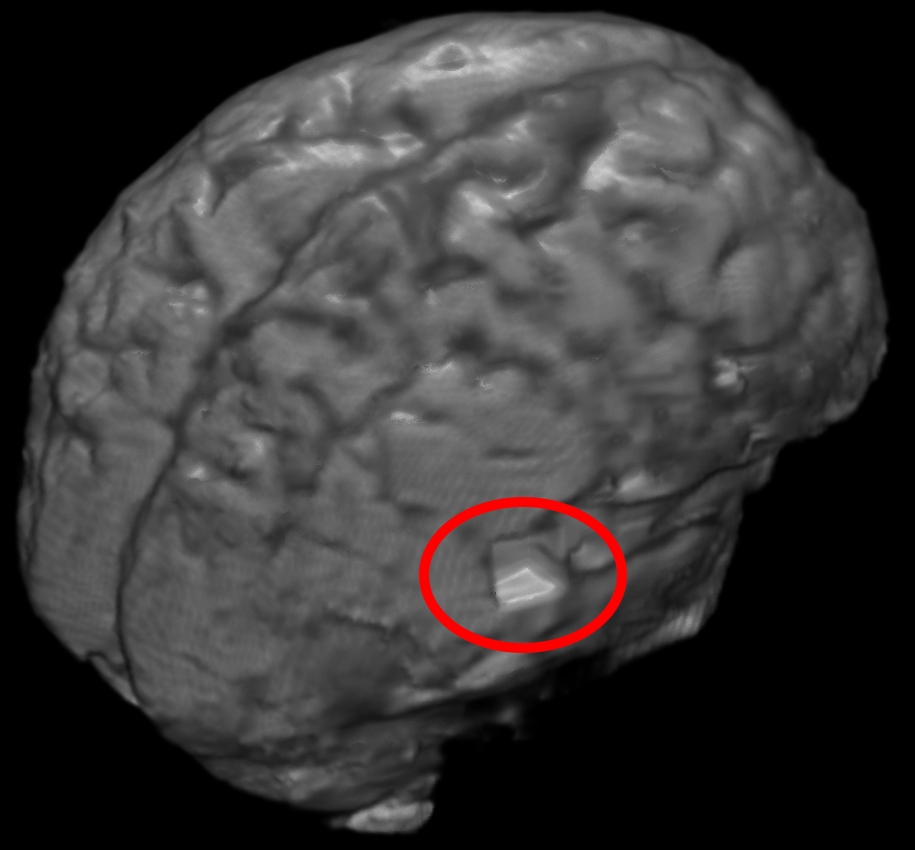
\includegraphics[width=8cm]{chapters/07_brats3d/images/brain-hdm-marked.png}
\caption{Modified scan with removed cube (red circle)}
\label{brats3d_example}
\end{figure}

\subsection{Docker execution}
\nblink{brats3D/03\_execute.ipynb}
To run the Docker container on all of our modified files, we have the correctly set up the directory that is mounted into the container. Similar to the 2D BraTS version, we want to analyze the impact of every modality separately. Do enhance the performance and avoid unnecessary file copying, we use filesystem hard links to prepare the directory. After running the Docker container on a single scan with only one modified modality, we copy away the result from the directory and update the directory content for the next execution.

Because of the long execution time for a single scan (1-2 minutes), we initially started a run with very big but few cubes cut out of the modality files. As expected, the output was very high coarse and did not provide much meaningful insight. We decided to execute the method with smaller cubes, but limited to one horizontal plane. The calculations for this configuration took around 6 hours on our current generation desktop machine with a high end consumer graphics card.

\subsection{Distance calculation}
\nblink{brats3D/04\_calculate\_hausdorff\_distance.ipynb}
The calculation of the distance between the ground truth segment and the output segment from the Docker containers are very similar to the 2D variant. The Hausdorff distance implementation we used only supports 2D matrices and not 3D volumes. A 3D implementation of the Hausdorff distance is feasible, but would be very slow with our volume size. 

Our solution was the following: We calculate the Hausdorff distance between all horizontal planes in the unchanged baseline network output and the corresponding plane in the ground truth segment.
This generates an array with a Hausdorff distance for every horizontal plane. We now do the same thing for all output segments generated from our modified scans. We then calculate the mean square error between the array from the baseline segment and the array from the current scan. This gives us a single value for every modified scan.

\subsection{Visualization}
Visualizing the calculated values is straight forward. We only run the algorithm on a single horizontal plane, we can therefore use 2D images to display the distances and the distances itself are saved in a 2D matrix. The distances correspond to a specific location, the location where a the cube has been taken out of the volume. We can convert the 2D matrix of the distances into an image (using a color map to convert the float values into a color gradient). As a last step, we upscale the generated image until it has the same size as the 2D plane on which it should be displayed.

\subsection{Results}
\nblink{brats3D/02a\_generate\_single\_slice.ipynb}
\nblink{brats3D/06\_display\_single\_slice.ipynb}

\begin{figure}[H]
    \centering
    \begin{subfigure}[t]{.32\textwidth}
        \centering
        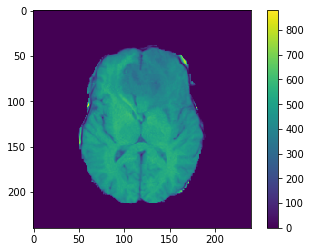
\includegraphics[width=\linewidth]{chapters/07_brats3d/images/01_t1.png}
        \caption{T1 modality of the slice}
    \end{subfigure}\hfill%
    \begin{subfigure}[t]{.315\textwidth}
        \centering
        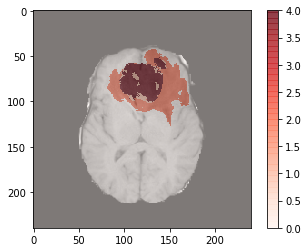
\includegraphics[width=\linewidth]{chapters/07_brats3d/images/05_t1_segment.png}
        \caption{T1 modality overlaid with ground truth tumor segment}
    \end{subfigure}\hfill%
    \begin{subfigure}[t]{.315\textwidth}
        \centering
        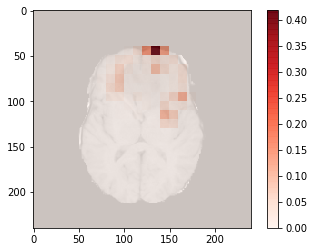
\includegraphics[width=\linewidth]{chapters/07_brats3d/images/09_t1_hdm10.png}
        \caption{T1 modality overlaid with Hausdorff distance mask output}
    \end{subfigure}
    \caption{Visualization of the Hausdorff distance mask result on the T1 modality.}
    \label{brats3d_t1}
\end{figure}

\begin{figure}[H]
    \centering
    \begin{subfigure}[t]{.32\textwidth}
        \centering
        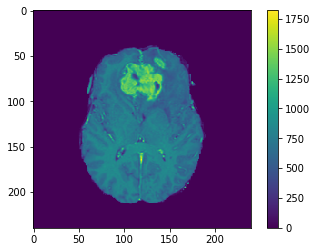
\includegraphics[width=\linewidth]{chapters/07_brats3d/images/02_t1ce.png}
        \caption{T1 contrast enhanced modality}
    \end{subfigure}\hfill%
    \begin{subfigure}[t]{.315\textwidth}
        \centering
        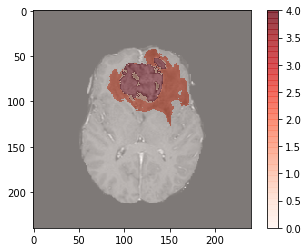
\includegraphics[width=\linewidth]{chapters/07_brats3d/images/06_t1ce_segment.png}
        \caption{T1ce modality overlaid with ground truth tumor segment}
    \end{subfigure}\hfill%
    \begin{subfigure}[t]{.315\textwidth}
        \centering
        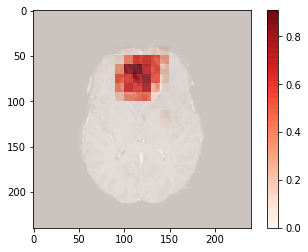
\includegraphics[width=\linewidth]{chapters/07_brats3d/images/10_t1ce_hdm.png}
        \caption{T1ce modality overlaid with Hausdorff distance mask output}
    \end{subfigure}
    \caption{Visualization of the Hausdorff distance mask result on the T1 contrast enhanced modality.}
    \label{brats3d_t1ce}
\end{figure}

\begin{figure}[H]
    \centering
    \begin{subfigure}[t]{.32\textwidth}
        \centering
        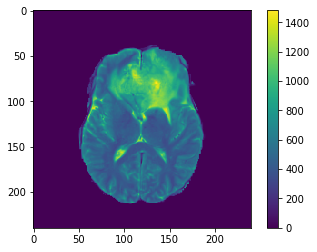
\includegraphics[width=\linewidth]{chapters/07_brats3d/images/03_t2.png}
        \caption{T2 modality of the slice}
    \end{subfigure}\hfill%
    \begin{subfigure}[t]{.315\textwidth}
        \centering
        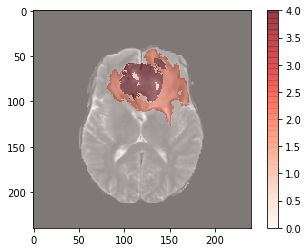
\includegraphics[width=\linewidth]{chapters/07_brats3d/images/07_t2_segment.png}
        \caption{T2 modality overlaid with ground truth tumor segment}
    \end{subfigure}\hfill%
    \begin{subfigure}[t]{.315\textwidth}
        \centering
        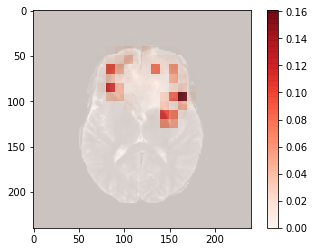
\includegraphics[width=\linewidth]{chapters/07_brats3d/images/11_t2_hdm.png}
        \caption{T2 modality overlaid with Hausdorff distance mask output}
    \end{subfigure}
    \caption{Visualization of the Hausdorff distance mask result on the T2 modality.}
    \label{brats3d_t2}
\end{figure}

\begin{figure}[H]
    \centering
    \begin{subfigure}[t]{.32\textwidth}
        \centering
        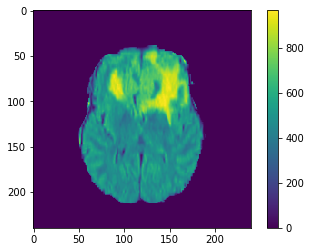
\includegraphics[width=\linewidth]{chapters/07_brats3d/images/04_flair.png}
        \caption{FLAIR modality of the slice}
    \end{subfigure}\hfill%
    \begin{subfigure}[t]{.315\textwidth}
        \centering
        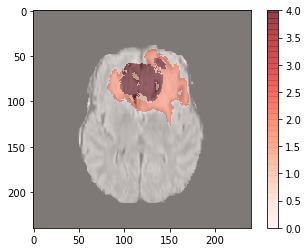
\includegraphics[width=\linewidth]{chapters/07_brats3d/images/08_flair_segment.png}
        \caption{FLAIR modality overlaid with ground truth tumor segment}
    \end{subfigure}\hfill%
    \begin{subfigure}[t]{.315\textwidth}
        \centering
        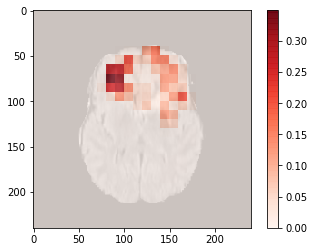
\includegraphics[width=\linewidth]{chapters/07_brats3d/images/12_flair_hdm.png}
        \caption{FLAIR modality overlaid with Hausdorff distance mask output}
    \end{subfigure}
    \caption{Visualization of the Hausdorff distance mask result on the FLAIR modality.}
    \label{brats3d_flair}
\end{figure}

\subsection{Discussion}
Figure \ref{brats3d_t1} shows the visualization of the distances when inserting cubes into the T1 modality. The marked regions in the visualization correspond mostly to the location of the tumor with some pixels outside of the tumor. Mauricio Reyes commented on this and said that there is discussion in the medical imaging community that the T1 modality is less useful for the segmentation of a tumor, and this result seems to support this argument.

Figure \ref{brats3d_t1ce} shows the visualization of the distances when inserting cubes into the T1 contrast enhanced modality. This contrast enhanced modality clearly shows the gadolinium enhanced tumor tissue, and from the output of the distances it looks like the neural network learned this fact and successfully uses it to generate a correct segmentation.

Figure \ref{brats3d_t2} shows the visualization of the distances when inserting cubes into the T2 modality. This modality displays the all tissue types in a similar way, but this neural network seems to use only the information for the edema of the tumor. Possibly because the T1 contrast enhanced modality provides higher quality data for the tumor core.

Figure \ref{brats3d_flair} shows the visualization of the distances when inserting cubes into the FLAIR modality. The FLAIR modality highlights the whole tumor, but places a 


\subsection{Conclusion}
shit works yo